
\documentclass[fleqn]{article}
\usepackage{amsmath}
\usepackage{graphicx}
\usepackage{booktabs}
\usepackage{float}
\usepackage{caption}
\usepackage{polynom}
\usepackage{mdwlist}
\usepackage{cancel}
\usepackage{fullpage}

\usepackage{parskip}
\usepackage{paralist}

\usepackage{unitsdef} 
\newunit{\inch}{in}
\newunit{\mile}{mile}
\newunit{\mph}{mph}
\newunit{\foot}{ft}
\newunit{\knot}{knot}
\newunit{\gallon}{gallon}

\setcounter{tocdepth}{2}

\everymath{\displaystyle}


% \begin{figure}[H]
%   \centering
%   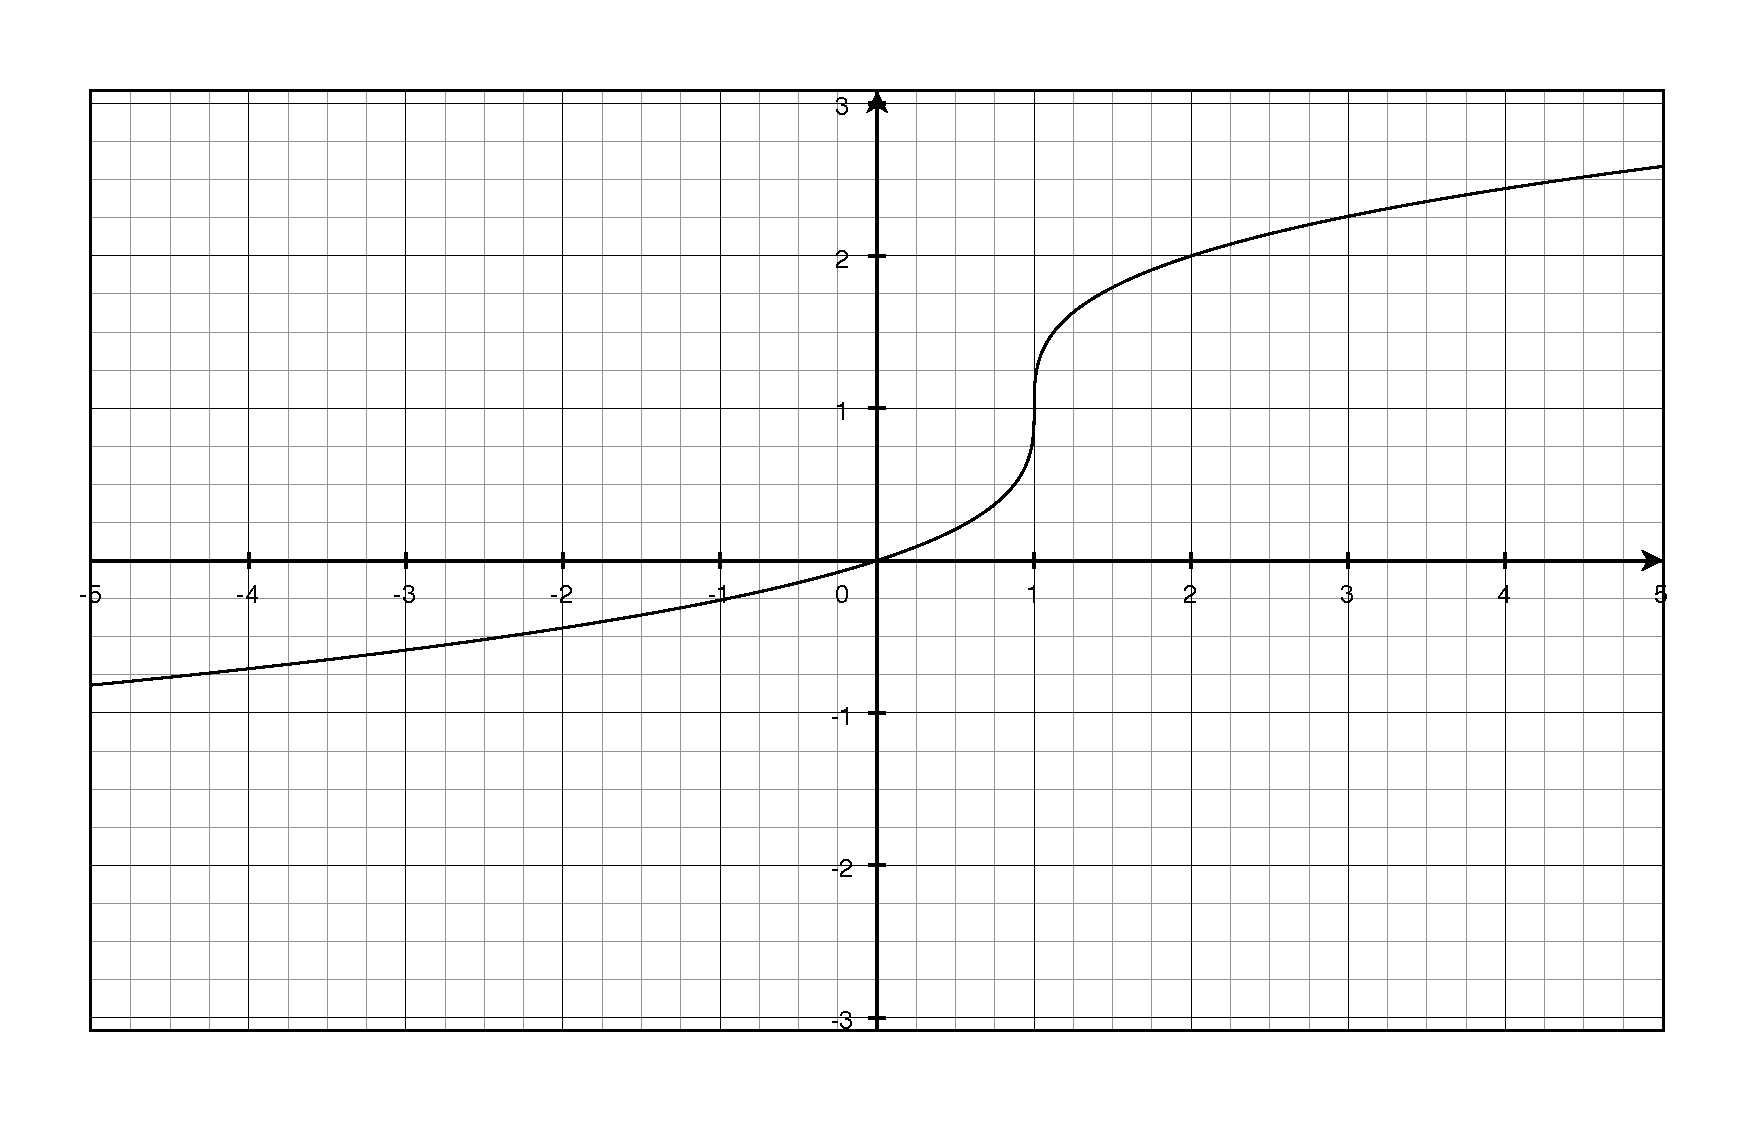
\includegraphics[scale=.3]{question7.eps}
%   \caption*{Question 7}
% \end{figure}

% \begin{tabular}{cc}
% \toprule
% period & amplitude \\
% \midrule
%   $\pi$ & $2$ \\
% \bottomrule
% \end{tabular}


%% \ifprintanswers
%% \usepackage{2in1, lscape}
%% \fi

\title{Math 263A Final Exam\\ Study Guide}
\date{June 6, 2012}

\author{}

\begin{document}

\maketitle  


\tableofcontents

\section{Disclaimer}

I made this study guide without access to the text book.  I tried to remember everything we covered, but I may
have forgotten a few things.  Your actual mileage may vary.

\section{General Suggestions}

\subsection{Test Taking Tips}
\begin{itemize}
\item Try hard not to leave any question blank.  Graders will usually give partial credit if you make some headway
  towards a solution.  If the test only has seven questions and you leave one blank, you definitely won't get an A and
  you'll need to do extremely well on everything else just to pass.

  If the question provides an equation, differentiate it, even if you don't know what to do next.  Differentiating is
  likely to be one of the steps towards the solution, so you should get some partial credit.

  If the question is a word problem, try to come up with some equation that uses the numbers from the problem and
  minimize/maximize, etc. (whatever is asked for in the problem).  Solve the problem with the equation you came up with,
  even if you're not confident the equation is correct.

\item Double check all your answers.  It's easy to make an arithmetic mistake, and I almost never get through the
  homework without making some careless mistakes.

\item Don't spend too much time on any question until you've at least looked at them all.  If you're stumped by
  something, make a note of it and come back to it at the end if you have time.


\end{itemize}

\subsection{Study Suggestions}
\begin{itemize}
  \item Do the practice test, obviously.  Make it realistic by doing it on your own with a time limit.

  \item Make your own practice test by selecting similar problems from the book, writing them down, and then doing them
    with a time limit.  Choose odd numbered problems so you can grade the test after you are done.  Repeat until you can
    consistently get at least 90\% on your sample tests.

  \item Practice each type of problem until you can solve that type of problem without thinking about it much.  Math is
  like playing a musical instrument.  If a musician goes to a performance knowing that he can play everything he's
  trying to play most of the time if he's a bit lucky, he's in trouble.  To perform well, he needs to be able to
  consistently play everything on the program really well without thinking about it much.

  The same is true for a math test.  If you can eventually figure out every type of problem with some effort, you're in
  trouble.  If you immediately know how to do every type of problem because you've practiced many similar problems,
  you're in good shape.

  \item For this course, there are a few common types of word problems, with some variations.  If you know how to do each type, and
  how to recognize which type you have, you should be fine.  The most common types are described in Sections
  \ref{related-rates} and \ref{min-max}.

  For any word problem, always draw a picture and label the parts.  Look for triangles, squares, or circles, and try to
  find equations using the Pythagorean Theorem, area formulas, etc.

  \item Do all the odd numbered word problems.  Check your answers.  Do them again until they are all routine.  There
    aren't that many types of word problems for this subject, so any problem you see on the final is likely to be the
    same as one from the book with different numbers.  
\end{itemize}

\section{Limits}
If you are taking the limit of the quotient of two polynomials and both the numerator and the are zero at the limit, try
to factor both polynomials.  If they have a common factor which cancels, the desired limit exists.

If you are taking an infinite limit of a quotient, there are three possibilities:
\begin{itemize*}
  \item the degree of the numerator and degree of the denominator are equal.  In this case the limit is the ratio of the
    leading coefficient of the numerator and denominator polynomials.
  \item the degree of the numerator is greater than the degree of the denominator.  In this case the limit is infinity
    or negative infinity.  The numerator grows much more rapidly than the denominator.

  \item the degree of the numerator is less than the degree of the denominator.  In this case the limit is zero.
    The numerator grows much less rapidly than the denominator.
\end{itemize*}

\section{Differentiation Rules}

You should know all the differentiation rules.  Fortunately, there aren't that many of them.  This section describes
them all.

It isn't enough to just know all the rules.  You should also practice them all so that you don't have to think about
them much, and they are all routine.  You need to do quite a few derivatives on the test, so you don't want to waste a
lot of time thinking about how to do each one.

\subsection{Power Rule}

\subsubsection{Rule}
\[
  D_x x^n = n x^{n - 1}
\]

The power rule applies, regardless of whether the thing raised to a power is a single variable or some more complicated
expression.  If it is anything more complicated than a single variable, you also have to apply the chain rule.

The power rule applies, even when the exponent is not a positive integer.  The exponent can also be negative and/or a
fraction and the same rule applies.

\subsubsection{Examples}

\begin{align*}
  D_x (x^5) &= 5x^4 \\
  D_x (3 x^5) &= 15x^4 \\
  D_x \left[ (x^2 + 1)^5 \right] &= 5 (x^2 + 1)^4 \cdot D_x (x^2 + 1) = 10x(x^2 + 1)^4 \\
\end{align*}


\subsection{Addition Rule}

\subsubsection{Rule}
\[
  D_x (u + v) = u' + v'
\]

You use this rule so frequently that you don't really think of it as a rule.

\subsubsection{Examples}

\begin{align*}
  D_x (2x^5 + 3x^2) &= 10 x^4 + 6x \\
  D_x (\sin x + \cos x) &=  \cos x - \sin x \\
\end{align*}


\subsection{Product Rule}
\subsubsection{Rule}
\[
  D_x (uv) = uv' + vu'
\]

$u$ and $v$ are functions of $x$.

\subsubsection{Examples}
\begin{align*}
  D_x \left[ x^2(x + 1)^3 \right] &= x^2 \cdot 3(x + 1)^2 + (x + 1)^3 \cdot 2x = (x + 1)^2(5x^2 + 2x) \\
  D_x (\sin x \cos x) &= \sin x \cdot (- \sin x) + \cos x \cdot \cos x \\
    &= \cos^2 x - \sin^2 x \\
\end{align*}

\subsection{Quotient Rule}
\subsubsection{Rule}

\[
  D_x \left( \frac{u}{v} \right) = \frac{vu' - uv'}{v^2}
\]

$u$ and $v$ are functions of $x$.

\subsubsection{Examples}
\begin{align*}
  D_x \left( \frac{x^3}{x^2 + 1} \right) &= \frac{(x^2 + 1) \cdot 3x^2 - x^3 \cdot 2x}{(x^2 + 1)^2} = \frac{x^4 + 3x^2}{(x^2 + 1)^2} \\
  D_x \left( \frac{\sin x}{\cos x} \right) &= \frac{\cos x \cdot \cos x - \sin x \cdot (- \sin x)}{\cos^2 x} \\
      &= \frac{1}{\cos^2 x} \\
      &= \sec^2 x \\
      &= D_x \tan x \\
\end{align*}

\subsection{Chain Rule}
\subsubsection{Rule}
\[
  D_x u(v(x)) = \frac{du}{dv} \cdot \frac{dv}{dx}
\]

$u$ and $v$ are functions of $x$.

This rule is called the chain rule because you can use it to chain together more than two functions.

The book describes rewriting the original function as two different functions, taking the derivative of these
separately, and then putting the result back together.  I find this technique to be error-prone and not very helpful, so
I don't use it---I just work from the outside in.  

Heres what I do:
\begin{itemize*}
\item If necessary, add extra parentheses to help correctly identify the outermost function.
\item Do one step of the chain at a time, writing down the each intermediate step.
\end{itemize*}


\subsubsection{Examples}
\begin{align*}
  D_x \left[ (2x^2 - 1)^5 \right] &= 5 (2x^2 - 1)^4 \cdot 4x = 20x (2x^2 - 1)^4 \\
  D_x \left( \sin^5 (x^2 + 1)^3 \right) &= D_x \left[ \left( \sin (x^2 + 1)^3 \right)^5 \right] \\
      &= 5 ( \sin (x^2 + 1)^3 )^4 \cdot D_x \sin (x^2 + 1)^3 \\
      &= 5 \sin^4 (x^2 + 1)^3 \cdot \cos (x^2 + 1)^3 \cdot D_x (x^2 + 1)^3 \\
      &= 5 \sin^4 (x^2 + 1)^3 \cdot \cos (x^2 + 1)^3 \cdot 3 (x^2 + 1)^2 \cdot D_x (x^2 + 1) \\
     &= 5 \sin^3 (x^2 + 1)^3 \cdot \cos (x^2 + 1)^3 \cdot 3 (x^2 + 1)^2 \cdot 2x \\
      &= 30x \cdot \sin^3 (x^2 + 1)^3 \cdot \cos (x^2 + 1)^3 \cdot (x^2 + 1)^2 \\
\end{align*}

The second example is more complicated than anything you're likely to see on the final, I think.  But it shows a
systematic procedure for unraveling a long chain.

\subsection{Trigonometric Functions}

The only two trigonometric functions you need to know the derivative of are sine and cosine.  If you know these two, you
can use the quotient rule to get any of the other derivatives you need.  

\begin{align*}
  D_x \sin x &= \cos x \\
  D_x \cos x &= - \sin x \\
\end{align*}

\section{Implicit Differentiation}
Sometimes it's difficult or impossible to solve an equation with two variables for one of the variables.  When this
happens you can use {\em implicit differentiation}.  The procedure is:

\begin{itemize*}
  \item differentiate both sides, treating $y$ as a function.
  \item solve for $\frac{dy}{dx}$.
\end{itemize*}

Usually both $x$ and $y$ appear in the final equation.  This means that you have to have values for both to get a result
for $\frac{dx}{dy}$.  This is fine if you need the value of the derivative at a particular point.

\section{Related Rates}
\label{related-rates}

\subsection{Moving Objects}

If you see a problem with two objects moving at right angles to each other and are asked to find the rate at which the
distance between them is changing, you have a {\em Moving Objects Related Rate} problem.  The objects might be cars,
boats, planes, walking people, dogs, etc.

Other problems which use exactly the same math but seem different at first are:
\begin{itemize}
\item A kite traveling horizontally at a fixed horizontal speed and height.  In this case, $\frac{dy}{dt} = 0$ (no
  change in height), and you need to find either $\frac{dr}{dx}$ (rate of change of string length) or $\frac{dx}{dt}$
  (horizontal speed).
\item An airplane traveling overhead at a fixed altitude.  This is the same as the kite problem with an airplane instead
  of a kite.
\end{itemize}

The key parts of this type of problem are:
\begin{itemize*}
\item Often the objects start moving at different times.
\item Often the objects are moving at different speeds.  Sometimes one of the objects is stationary.
\item If both objects are moving, one object is moving along the x axis and the other object is moving along the y axis.
\end{itemize*}

The final equation for this type of problem generally looks like this:
\[
  \frac{dr}{dt} = \frac{y}{r} \cdot \frac{dy}{dt} + \frac{x}{r} \cdot \frac{dx}{dt}
\]

This equation makes sense:
\begin{itemize}
  \item If $\frac{y}{r} \approx 1$, then $\frac{x}{r} \approx 0$ and most of the change in the total distance comes from
    the y direction.  For example if one car is in Portland heading towards Los Angeles and the other is in Seattle
    heading towards Yakima, most of the change in distance between the two cars comes from the Portland car.

  \item if $\frac{dy}{dt}$ is a lot bigger than $\frac{dx}{dt}$, then the y speed affects the total more than the x
    speed.  For example if a car and a bicycle start out together in Seattle, with the car going south and the bike
    going east, most of the change in the distance between them comes from the car.
 
\end{itemize}

The steps for solving this type of problem are:
\begin{itemize*}
  \item Have one object move along the x axis and the other object move along the y axis
  \item Find expressions for x and y in terms of time.  Be careful about the direction (positive or negative) each
    object is moving in
  \item Let $r$ be the distance between the two objects
  \item Use the Pythagorean theorem to find an expression for $r^2$ in terms of $x$ and $y$.  $r^2$ is usually better
    than $r$ because it makes the differentiation easier.
  \item Use implicit differentiation to get the expression shown above.
  \item Substitute in the rates and distances you have and solve for the missing rate.
\end{itemize*}

\subsection{Volume}

You have some oddly shaped object which is gradually being filled with water.  You know the rate the volume is changing
(the rate the water is going in) and want to know the rate the height is changing.  The steps are:

\begin{itemize*}
\item write down all the equations you can think of for height, width, radius, volume, etc.
\item find an expression for the volume in terms of just one height/width/radius variable by solving one of the other
  equations for one of these and substituting it in the volume equation
\item use implicit differentiation to get $\frac{dV}{dt}$ in terms of $\frac{dh}{dt}$, etc.
\item plug in the values you know and solve for whatever you are missing
\end{itemize*}

\section{Minimization/Maximization}
\label{min-max}

\subsection{General}

\begin{itemize}
  \item If you are asked to find the min/max over a closed (with square brackets) interval, you need to check whether
    either of the end points is a min/max.
  \item Don't include the end points if you are looking in an open (with parentheses) interval.
  \item A {\em local min/max} is a point which is smaller/larger than its immediate neighbors but not necessarily
    smaller/larger than all the other points.
  \item You can find local min/max by:
    \begin{itemize*}
      \item find the first derivative
      \item set to 0 and solve to find candidate points
      \item also look for places where the first derivative is undefined or infinite
      \item for each candidate point, you have several possibilities.
        \begin{itemize*}
          \item check whether the second derivative is positive or negative.  A positive second derivative is a local min
            and a negative second derivative is a local max.
          \item check whether the first derivative goes from negative to positive or positive to negative at this
            point.  If the function was increasing before and decreasing after, you have a local max, and vice versa.
          \item If you are looking over a specific interval, plug in values, including the end points
        \end{itemize*}
        If you have time and there's more than one way to do it, try two ways and make sure they agree
    \end{itemize*}
\end{itemize}

\subsection{Area/Perimeter}

In an area/perimeter, you are trying to build some sort of usually-oddly-shaped enclosure with some constraint on the
materials used.  Examples are:

\begin{itemize*}
\item build the maximum area pen with an interior divider and a fixed amount of fence
\item build the maximum area rectangular pen with one side provided by a river
\item build the cheapest pen with a specified area and some constraint on the cost of the building materials
\end{itemize*}

To solve this kind of problem:
\begin{itemize*}
\item Draw a picture of the situation.  
\item Label the sides, radius, etc., with variables
\item Get as many equations as you can out of the picture.  The equations may involve cost, area, or perimeter.  Usually
  there will be more than one equation.  One of the equations will always be for the quantity you are trying to minimize
  or maximize.

\item If the equation for the quantity you are trying to maximize has more than one variable in it, you have a problem.
  You can't optimize for two things at once, so you need to get rid of one of the variables.  Do this by:
  \begin{itemize*}
    \item solve another equation for a variable you'd like to get rid of
    \item substitute the result in the first equation  
  \end{itemize*}

\end{itemize*}

Now you have an equation for the quantity you are interested with one variable, and the hard part is over.  To optimize:
\begin{itemize*}
  \item take the derivative
  \item set the resulting equation to zero
  \item solve
\end{itemize*}

This will give you one or more critical values.  To find if any of the candidates are actually maximums or minimums:
\begin{itemize*}
  \item Plug them in the equation and get values
  \item Plug the value of the ends of the range and get values.  It's possible that the best thing to do, for example,
    is to not use any of the expensive fence and build the enclosure entirely out of cheap fence, or something like
    that.
  \item Whichever of these numbers is best is the answer.
\end{itemize*}

If plugging all the numbers into the equation is difficult and time consuming, you can also use the second derivative
test to see if the critical points are minimums or maximums.

\subsection{Surface Area/Volume}
Another common optimization problem is area/volume.  These problems are often disguised as amount of materials/volume or cost/volume.
Minimizing the amount of materials required to build a container of a particular
shape and specified volume really amounts to minimizing the area of the container, given a desired volume.

Example of this type of problem are:
\begin{itemize*}
  \item Find the dimensions of the minimum cost rectangular box with volume $1 \meter^3$ when the materials used for the top and bottom
    cost twice as much as the materials used for the sides.
  \item Find the dimensions which minimize the amount of metal required to construct a $1 \meter^3$ metal container with a cylindrical base and
    hemispherical top.
\end{itemize*}

The steps for this type of problem are:
\begin{itemize*}
\item Draw a picture of the container.
\item Write equations for the area and volume.  Sometimes you need to think of the container in two pieces and add the
  results together.  For example, if your container is a cylinder with a hemispherical base, write equations for a
  cylinder and for a hemisphere, and add them together.
\item If the area equation involves more than one variable, as it usually does:
  \begin{itemize*} 
    \item solve the volume equation for one of the variables
    \item substitute the result in the area equation
  \end{itemize*} 
\end{itemize*}

\section{Graphing}

Calculus provides some helpful tools for drawing graphs.  There is a checklist of things to do, each of which helps give
you a clearer picture of the final graph.  Some of the things you already know from pre-calculus.  Here's the full list:

\subsection{Symmetry}

To determine if there is any symmetry, find $f(-x)$.  

If $f(-x) = f(x)$, the function is {\em even} and has y-axis symmetry.  This is nice because you only need to draw the right
half of the graph.  The left half will be a reflection of the right.

If $f(-x) = -f(x)$, the function is {\em odd} and has origin symmetry.

If neither of these is true, which is usually the case, there isn't any symmetry.

\subsection{First Derivative Test}
\label{first-derivative-test}

Find $f'(x)$ and figure out where it is 0, undefined, negative, and positive.  

The points where $f'(x) = 0$ are {\em critical points}.  These are places where the function might change direction.
The points where $f'(x)$ is undefined are points where either $f(x)$ is undefined, or where $f(x)$ makes a sharp point
or vertical line.  These are also places where the function might change direction.

Critical points are also potential minimums and maximums for the function.  You can determine if one of these values is
actually a minimum or maximum by either:

\begin{itemize*}
  \item If $f'(x)$ has different signs before and after the point, it is a minimum or maximum
  \item If $f''(x) \neq 0$ at this point, it is either a minimum or maximum.  A positive second derivative indicates a
    minimum and a negative second derivative indicates a maximum.
\end{itemize*}

Where $f'(x) > 0$ the original function is increasing.

Where $f'(x) < 0$ the original function is increasing.

\subsection{Second Derivative Test}

Find $f''(x)$ and figure out where it is 0, undefined, negative, and positive.  

The points where $f'(x) = 0$ are {\em inflection points}.  These are places where the function might change shape.

The points where $f''(x)$ is undefined are points where either $f'(x)$ is undefined, or where $f'(x)$ makes a sharp point
or vertical line.  These are also places where the function might change shape.

Where $f''(x) > 0$ the original function is {\em concave up}.

Where $f''(x) < 0$ the original function is {\em concave down}.

The second derivative is also useful in identifying minimums and maximums as described in Section \ref{first-derivative-test}.

\subsection{Limits at Infinity}
If $\lim_{x \to \pm \infty} = c$, then there is a horizontal asymptote at c.

\subsection{Infinite Limits}
If $\lim_{x \to c} = \pm \infty$ then there is a vertical asymptote at c.

\subsection{Drawing the Graph}
Once you have done all the preceding steps, you should have a fairly good picture of the graph.  Select a few key
points, plug the x values into the graph to get the y-values, and draw the graph.

When you are doing this, make sure that the values agree with the shapes, min/max, etc. that you found from earlier
steps.  If they don't agree, something is wrong.  Go back and check your earlier work and check the values until you
figure out what is wrong.

\section{Miscellaneous}
\begin{itemize}
\item {\em differentials} can be used to estimate an approximate value.  Review the appropriate section in the book.
\item The {\em Mean Value Theorem} says that when traveling between two points, your actual instantaneous speed must at
  some point during the trip be equal to your average speed during the trip, as long as:
  \begin{itemize*}
    \item your speed is defined and finite at every point ($f$ is differentiable)
    \item you don't jump through hyperspace to get from one point to another ($f$ is continuous)
  \end{itemize*}
\end{itemize}

\end{document}
